%!TEX root = ../main.tex
\chapter{Le projet et de son impacte sur les équipes}
Comme pour tout projet lié à des éléments de l'architecture informatique d'une entreprise, la sécurisation de la chaîne
de production d'applications conteneurisées à un impacte sur différentes équipes de l'entreprise. Cet impacte est présent
tant lors de la mise en place du projet que lors des la phase opérationnelle faisant suite à la livraison du projet.

Nous chercherons donc dans ce chapitre à évaluer cet impacte sur les équipes du Groupe ainsi que les éventuelles 
difficultés rencontrées durant la réalisation de ce projet.

\section{Rappel de contexte}
Comme évoqué dans les précédemment chapitres, cette mission de fin d'étude et le projet associé s'est déroulé
durant la crise de la COVID-19, plus particulièrement du la \textit{3ème vague épidémiologique}. Cette crise ayant un 
impacte mondiale, les activités du Groupe JCDecaux ont significativement chutés. Une majorité des unités organisationnelles
ont donc vue leur activité réduite à divers pourcentages.

Cette réduction d'activité, à hauteur de 30\% pour la \ac{DSI} Groupe, et les départs liés aux deux plans de conservation
de l'emplois ont eu pour effet de mettre en tension les équipes de la \ac{DSI}. Ainsi, si en théorie cette mission est
censé représenter six mois de travail, dans les fait elle représent un peu plus de trois mois effectifs.
\newline De plus, l'activité de l'équipe sécurité ainsi que celle des autres équipes impacté par ce projet n'étant pas 
pas arrêter mais modérément diminué, ce projet ne pouvais occuper 100\% du temps de travail.

Ces éléments expliquent donc la durée de réalisation de cette mission qui, à mon sense, aurait pu être réalisé en 
quatres mois dans des conditions plus favorables.

\section{Estimation des charges et retroplanning}
Ce projet a été réalisé en deux phases successives : une première phase visant à entériner la procédure de qualification 
sécurité des applications puis une deuxième visant à sécuriser les conteneur et leur déploiement sur \ac{K8S}.
\newline Plusieurs équipes de la \ac{DSI} ont participés à la réalisation de ce projet conjointement avec l'équipe de 
\ac{SSI}.

\newpage

La charge pour ces équipes pour chaque grandes étapes du projet est estimée comme suivant :
\begin{enumerate}
    \item Processus d'audit :
    \begin{itemize}
        \renewcommand{\labelitemi}{•}
        \item Équipes de développement France : 13 équ. Heure/Homme
    \end{itemize}
    \item Sécurisation des clusters \ac{K8S} :
    \begin{itemize}
        \renewcommand{\labelitemi}{•}
        \item Équipe d'architecture : 27 équ. Heure/Homme
        \item Équipe d'infrastructure : 5 équ. Heure/Homme
    \end{itemize}
    \item Politique de sécurité \ac{K8S} :
    \begin{itemize}
        \renewcommand{\labelitemi}{•}
        \item Équipe d'architecture : 3 équ. Heure/Homme
        \item Équipes d'infrastructure : 6 équ. Heure/Homme
    \end{itemize}
    \item Revue des vulérabilités des conteneurs :
    \begin{itemize}
        \renewcommand{\labelitemi}{•}
        \item Équipes d'architecture : 1 équ. Heure/Homme
        \item Équipes d'infrastructure : 5+ équ. Heure/Homme
    \end{itemize}
\end{enumerate}

Cette mission de fin d'étude ne disposant pas de réelles contrainte temporelles, seul quelques jalons ont étés proposés.
C'est pourquoi j'ai réalise un rétroplanning afin de vous présenter la chronologie du projet.

\begin{figure}[h]
    \centering
    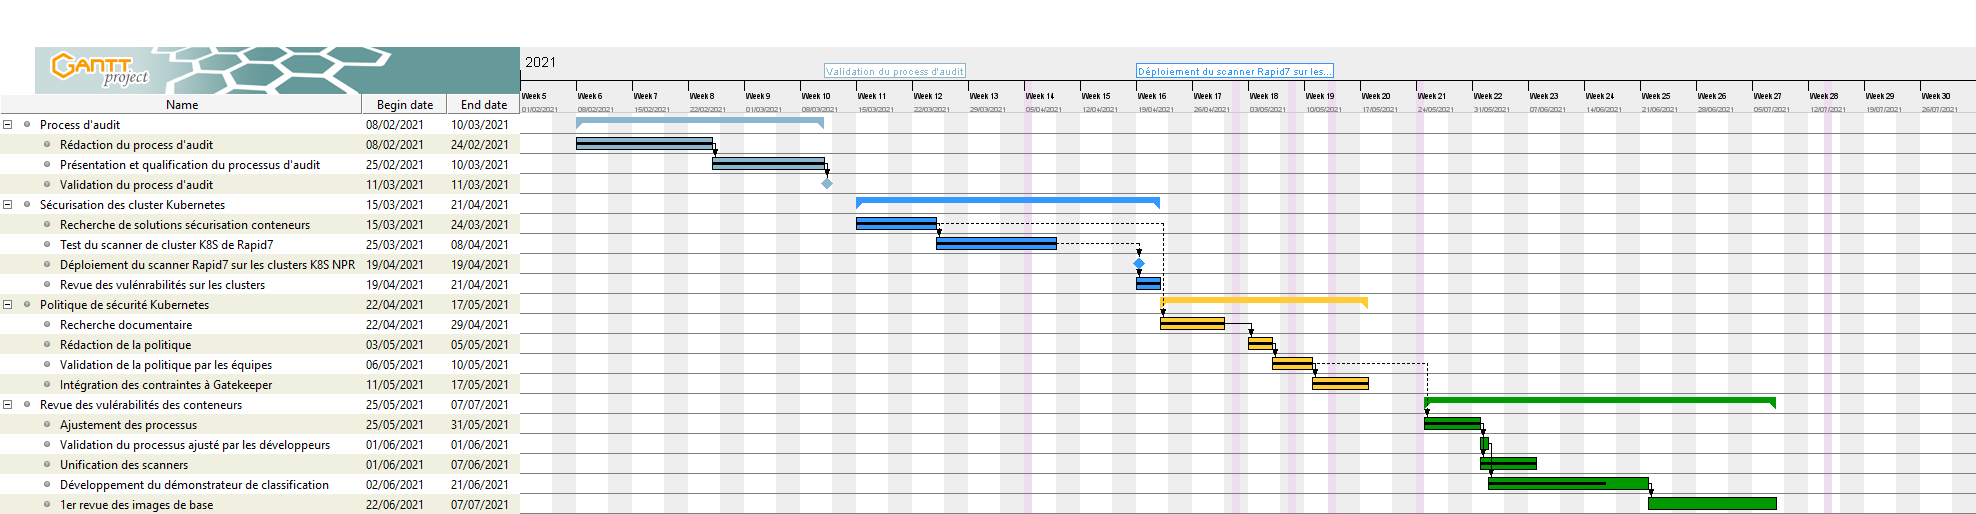
\includegraphics[width=\linewidth]{resources/img/retroplanning.png}
    \caption{Rétroplanning de la mission de fin d'étude}
\end{figure}

\begin{center}
    \colorbox{gray!15}{Une version plus lisible est disponible dans les annexes}
\end{center}